\documentclass[a4paper]{article}

\usepackage[T1]{fontenc}
\usepackage{textcomp}
\usepackage{mathtools,amssymb,amsthm}
\usepackage[hmargin=1in,vmargin=1in]{geometry}
\usepackage{graphicx,cancel}
\usepackage[math-style=TeX]{unicode-math}
% \usepackage[lite,subscriptcorrection,nofontinfo]{mtpro2}
\usepackage{fontspec}
\usepackage[colorlinks=true,allcolors=blue]{hyperref}

\defaultfontfeatures{Ligatures=TeX,Numbers=OldStyle}
\setmainfont{Palatino Linotype}
\setmathfont{TeX Gyre Pagella Math}
%\usepackage[integrals]{wasysym}
\frenchspacing

\newcommand*{\parasp}{\setlength{\parskip}{10pt plus 2pt minus 3pt}}
\newcommand*{\noparasp}{\setlength{\parskip}{0pt plus 1pt}}
\newcommand*{\setparasp}[1]{\setlength{\parskip}{#1}}
\newcommand*{\pskip}{\vskip 10pt plus 2pt minus 3pt}
\newcommand\LEFTRIGHT[3]{\left#1 #3 \right#2}
\newcommand*{\paren}[1]{\LEFTRIGHT(){#1}}
\newcommand*{\brkt}[1]{\LEFTRIGHT[]{#1}}
\newcommand*{\unit}[1]{\,\mathrm{#1}}
\newcommand*{\DeclareUnit}[2]{\newcommand*{#1}{\unit{#2}}}
\DeclareUnit{\cm}{cm}
% \renewcommand*{\m}{\unit{m}}
\DeclareUnit{\m}{m}
\DeclareUnit{\kg}{kg}
\DeclareUnit{\s}{s}
\newcommand*{\R}{\mathbb{R}}
\newcommand*{\Rp}{(0,+\infty)}
\newcommand*{\Rm}{(-\infty,0)}
\newcommand*{\deduce}{\mathrel{\Downarrow}}
\newcommand*{\abs}[1]{\left\lvert #1 \right\rvert}
\newcommand*{\reason}[1]{\langle \, \text{#1} \, \rangle}

\newcounter{ListCounter}
\newenvironment{enumerate*}%
{\begin{list}%
        {\arabic{ListCounter}.}%
        {\usecounter{ListCounter}%
            \setlength{\topsep}{1.5pt}%
            \setlength{\itemsep}{1.5pt} } }%
    {\end{list}}

\DeclareMathOperator{\arccosh}{arccosh}
\DeclareMathOperator{\gammaf}{\Gamma}
\DeclareMathOperator{\var}{var}
\DeclareMathOperator{\Ber}{Bernoulli}
\DeclareMathOperator{\Cov}{Cov}
\DeclareMathOperator{\E}{E}
%\newcommand*{\diff}{\mathop{}\!d}
\newcommand*{\diff}{\mathop{}\!\mathit{d}}
%\newcommand*{\diff}{\mathop{}\!\mathrm{d}}
\newcommand*{\dx}{\diff x}
\newcommand*{\dy}{\diff y}
\newcommand*{\dz}{\diff z}
\newcommand*{\dt}{\diff t}
\newcommand*{\du}{\diff u}
\newcommand*{\dv}{\diff v}
\newcommand*{\dtheta}{\diff \theta}
\newcommand*{\ddx}{\frac{\diff}{\dx}}
\newcommand*{\fwdf}{\mathop{}\!\Delta}
\newcommand*{\dydx}{\frac\dy\dx}
\newcommand*{\pdpdx}{\frac\partial{\partial x}}
\newcommand*{\pdpdy}{\frac\partial{\partial y}}
\newcommand*{\pdpdz}{\frac\partial{\partial z}}
\newcommand*{\pdpdu}{\frac\partial{\partial u}}
\newcommand*{\pdpdv}{\frac\partial{\partial v}}
\newcommand*{\pdpdt}{\frac\partial{\partial t}}
\newcommand*{\pdzpdx}{\frac{\partial z}{\partial x}}
\newcommand*{\pdzpdy}{\frac{\partial z}{\partial y}}
\newcommand*{\pdzpdt}{\frac{\partial z}{\partial t}}
\newcommand*{\pdxpdt}{\frac{\partial x}{\partial t}}
\newcommand*{\pdypdt}{\frac{\partial y}{\partial t}}

\AtBeginDocument{%
	\renewcommand{\perp}{\mathrel{\bot}}
	\let\leq\leqslant
	\let\le\leq
        \let\geq\geqslant
        \let\ge\geq}

\newcommand*{\Prb}[1]{\section*{Problem #1}}
\newcommand{\Q}[1]{\textbf{Question:} #1}
\newcommand*{\A}[1]{\textbf{Answer:} #1}
\newcommand{\Prblm}[3]{\Prb{#1} \Q{#2} \\[6pt] \A{#3}}


\everymath{\displaystyle}

\title{\bf Solutions to Chapter 2 Quiz: Functions}
\author{Lei Zhao}
\date{}

\begin{document}
  \maketitle
  
  \Prblm{1}
    {If $f(x) = x^{2x}$, compute $\frac{df}{dx}$.}
    {$2x^{2x}(1 + \ln x)$.}
    \begin{align*}
      \ln( y &= x^{2x} ) \\
      d( \ln y &= 2x \ln x ) \\
      \frac{dy}{y} &= \paren{\frac{2x}{x} + \ln x} dx \\
      \frac{dy}{dx} &= y (1 + \ln x) \\
      \frac{dy}{dx} &= x^{2x} (1 + \ln x).
    \end{align*}
    
    {\parasp This problem tests your understanding of the topics in lecture 16
    \href{https://class.coursera.org/calcsing-007/lecture/314}{Differentiation
    Operator}. This is a function of super-exponential type.
    
    The function of the type $u(x)^{v(x)}$ in fact can be transformed into
    $e^{v(x) \ln u(x)}$, differentiate this and you get
    \[ \frac{d}{dx} u(x)^{v(x)} = u(x)^{v(x)} \paren{\frac{v(x)}{u(x)} u'(x) + 
    v'(x) \ln u(x)}. \] }
    
  \Prblm{2}
    {Consider the function $f(x) = \sqrt{3}x^2e^{1-x}$. Use the formula
    for curvature,
    \[\kappa = \frac{\lvert f'' \rvert}{( 1+|f'|^2 )^{3/2}}\]
    to compute the curvature of the graph of $f$ at the point $(1,
    \sqrt{3})$.}
    {$\frac{\sqrt{3}}{8}$.}
    \begin{align*}
      f'(x) &= 2\sqrt{3}xe^{1-x} - \sqrt{3}x^2e^{1-x} \\
        &= \sqrt{3}xe^{1-x}(2-x) \\
      f''(x) &= \sqrt{3}e^{1-x}(1-x)(2-x) - \sqrt{3}xe^{1-x} \\
        &= \sqrt{3}e^{1-x}[(1-x)(2-x)-x] \\
      f'(1) &= \sqrt{3} \\
      f''(1) &= -\sqrt{3} \\
      \kappa \,\Bigr\vert_{(1, \sqrt{3})}
        &= \frac{\sqrt{3}}{(1+3)^{3/2}}
        = \frac{\sqrt{3}}{8}.
    \end{align*}
  
  \Prblm{3}
    {Assume that $x$ and $y$ are related by the equation $y \ln x = e^{1-x}
    + y^3$. Compute $\frac{dy}{dx}$ evaluated at $x=1$.}
    {$0$.}
    \begin{align*}
      d( y \ln x &= e^{1-x} + y^3 ) \\
      \frac{y \, dx}{x} + \ln x \, dy &= -e^{1-x} \, dx + 3y^2 \, dy \\
      \frac{dy}{dx} &= \frac{\frac{y}{x} + e^{1-x}}{3y^2 - \ln x} \\
      \intertext{solve the original equation about $x = 1$ and get}
        x &= 1 \\
        y &= -1 \\
      \intertext{substitute $x$ and $y$ into the above formula about
      $\frac{dy}{dx}$ and get}
      \left.\frac{dy}{dx}\right\rvert_{(1,-1)}
        &= \frac{-1+1}{3} = 0.
    \end{align*}
  
  \Prblm{4}
    {Use the linear approximation of the function $f(x) = \arctan(e^{3x})$
    at $x=0$ to estimate the value of $f(0.01)$. \\
    \textbf{Hint:} remember that $\frac{d}{dx}\arctan(x) = \frac{1}{1+x^2}$.}
    {$\frac{\pi}{4} + \frac{3}{200}$.}
    \begin{align*}
      f(x+h) &\approx f(x) + f'(x)h \\
      f(0.01) &\approx f(0) + f'(0) \times 0.01 \\
      f(0) &= \frac{\pi}{4} \\
      f'(x) &= \frac{3e^{3x}}{1+e^{6x}} \\
      f'(0) &= \frac{3}{2} \\
      f(0.01) &\approx \frac{\pi}{4} + \frac{3}{200}.
    \end{align*}
  
  \Prblm{5}
    {A rectangular picture frame with total area $50000 \cm^2$ includes a
    border which is $1 \cm$ thick at the top and the bottom and $5 \cm$ thick
    at the left and right side. What is the largest possible area of a picture
    that can be displayed in this frame?}
    {$98 \cm \times 490 \cm$.}
    
    {\parasp $S$ is the total area of the picture being displayed by this frame
    and $x$ is the width of the top and bottom side of the rectangle that
    actually displays the picture (i.e.\ frame width minus the left and right
    border size). Similarly, the height of the left and right side of the
    rectangle displaying the picture is $50000/(x+10) - 2$. So
    \begin{align*}
      S &= \paren{\frac{50000}{x+10} - 2}x \\
        &= \frac{50000(x+10) - 500000}{x+10} - 2x \\
        &= 50000 - \frac{500000}{x+10} - 2x \\
      S' &= \frac{500000}{(x+10)^2} - 2.
    \end{align*}
    
    $x$ only makes sense when it's positive. $S'$ is monotonically
    decreasing on $(0,+\infty)$ and has a zero at $x=490$. Thus, $S'$ is
    positive on $(0,490)$ and negative on $(490,+\infty)$, and $S$ is
    monotonically increasing on $(0,490)$ and monotonically decreasing on
    $(490,+\infty)$. Therefore, $S$ has a maximum at $x=490$. At this time,
    the corresponding height is $50000/(490+10) - 2 = 98$. Hence, $98 \cm
    \times 490 \cm$.
    
    \begin{figure}[h]
      \centering
      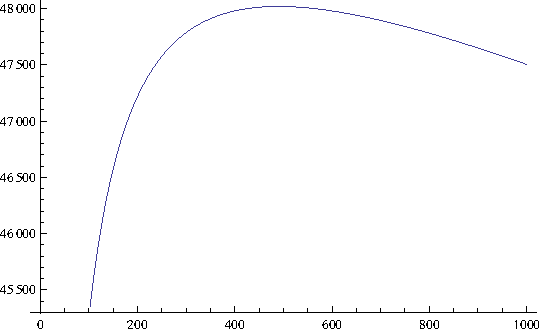
\includegraphics{quiz2_solved_fig1}
      \caption{the area $S$ with respect to $x$}
    \end{figure}
    
    \begin{figure}[h]
      \centering
      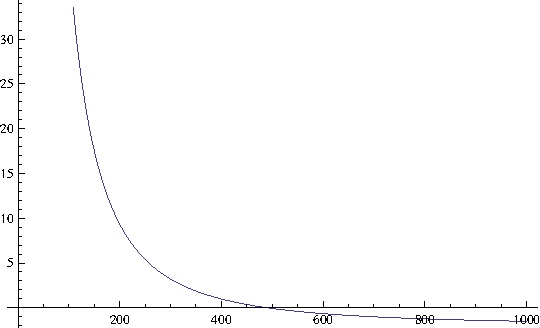
\includegraphics{quiz2_solved_fig2}
      \caption{the rate of change of area, $S'$, with respect to $x$}
    \end{figure}
    
    This is an optimization problem. Please refer to lecture 14
    \href{https://class.coursera.org/calcsing-007/lecture/310}{Optimization}.}
  
  \Prblm{6}
    {Which of the following statements are true for the function $f(x) =
    \frac{4}{x}+x^4$\,? In order to receive full credit for this problem, you
    must select all the true statements (there may be many) and none of the
    false statements.}
    {\begin{table}[h]
      \begin{tabular}{lcl}
          & a. & The global maximum of $f$ for $-3/2 \le x \le 2$ is at
          $x=-1$. \\
        \checkmark
          & b. & The global maximum of $f$ for $-2 \le x \le -1$ is at
          $x=-2$. \\
          & c. & The critical points of $f$ are at $x=-1$ and $x=1$. \\
        \checkmark
          & d. & The global maximum of $f$ for $-1 \le x \le -1/2$ is at
          $x=-1$. \\
          & e. & The global minimum of $f$ for $-2 \le x \le 2$ is at
          $x=1$. \\
        \checkmark
          & f. & $f$ is not differentiable at $x=0$. \\
        \checkmark
          & g. & The global minimum of $f$ for $1/2 \le x \le 2$ is at
          $x=1$. \\
          & h. & The global minimum of $f$ for $-1 \le x \le 2$ is at
          $x=1$. \\
      \end{tabular}
    \end{table}}
    
    {\parasp $f$ is not defined at $x=0$, and this hints us it has a
    blow-up or oscillation around $x=0$. In fact, $f$ is continuous
    everywhere except at $x=0$, and has a blow-up to positive infinity
    as $x \to 0^+$ and a blow-up to negative infinity as $x \to
    0^-$. So $f$ is not differentiable at $x=0$ and any intervals
    containing zero as its interior point have neither maximum nor
    minimum since $f$ can be arbitrary large toward both positive and
    negative infinity around $x=0$. Therefore, a., e., and h.\ are
    all incorrect and f.\ is correct.
    
    Take the derivative and we get $f'(x) = 4x^3 - 4/x^2$. The first term
    $4x^3$ has the same sign as $x$ and is monotonically increasing on \R,
    the second term $-4/x^2$ is always negative and monotonically
    increasing on \Rp; therefore, $f$ is always negative on \Rm{} and
    monotonically increasing on \Rp. $f'$ has a zero at $x=1$; and thus
    $f'$ is negative on $(0,1)$ and positive on $(1, +\infty)$. Therefore,
    $f$ is monotonically decreasing on $\Rm \cup (0,1)$ and monotonically
    increasing on $(1,+\infty)$. Hence, b., d., and g.\ are all correct.
    
    $f'(x) = 0$ when $x=1$ and $f'(x)$ doesn't exist when $x=0$. So
    the critical points of $f$ are at $x=0$ and $x=1$. Therefore, c.\
    is incorrect.}
    
    \begin{figure}[h]
      \centering
      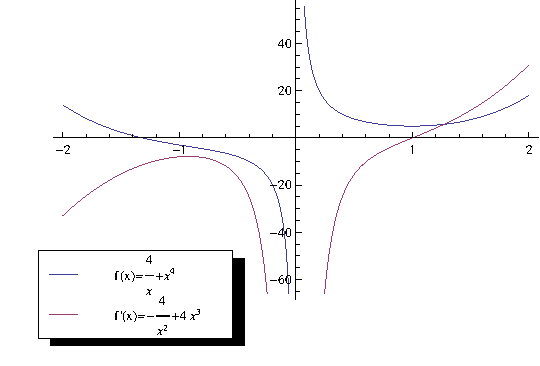
\includegraphics{quiz2_solved_fig3}
      \caption{The plot of $f$ and $f'$}
    \end{figure}
  
  \Prblm{7}
    {To approximate $ \sqrt[3]{15} $ (the cube root of $ 15 $) using Newton's
    method, what is the appropriate update rule for the sequence $ x_n $?}
    {$ x_{n+1} = \frac{2x_n}{3} + \frac{5}{x_n^2} $.}
    
    {\parasp $ \sqrt[3]{15} $ is the solution to the equation $ x^3 - 15 = 0 $.
    So let $ f(x) = x^3 - 15 $ and
    \begin{align*}
      x_{n+1} &= x_n - \frac{f(x)}{f'(x)} \\
      f'(x) &= 3x^2 \\
      x_{n+1} &= x_n - \frac{x_n^3 - 15}{3x_n^2} \\
      &= \frac{3x_n^3 - x_n^3 - 15}{3x_n^2} \\
      &= \frac{2x_n}{3} - \frac{5}{x_n^2}.
    \end{align*}
    
    Please refer to lecture 12
    \href{https://class.coursera.org/calcsing-007/lecture/296}{Linearization}.}
  
  \Prblm{8}
    {Fill in the blank:
    \[ \ln^2(x+h) = \ln^2 x + \underline{\qquad}\cdot h + O(h^2) \]
    Here, $ \ln^2 x $ means $ (\ln x)^2 $.}
    {$ 2\frac{\ln x}{x} $.}
    
    {\parasp The stronger version of derivative is defined by the second order
    variation. The above blank happen to be in the position of the second order
    variation, so it's just the derivative of $ \ln^2 x $, which is
    \[ (\ln^2 x)' = \frac{2\ln x}{x}. \]
    
    Please refer to lecture 10
    \href{https://class.coursera.org/calcsing-007/lecture/292}{Derivatives}.}
  
  \Prblm{9}
    {Recall that the kinetic energy of a body is
    \[ K = \frac{1}{2}mv^2 \]
    where $ m $ is mass and $ v $ is velocity. Compute the relative rate of
    change of kinetic energy, $ \frac{dK}{K} $, given that the relative rate of
    change of mass is $ -7 $ and the relative rate of change of velocity is
    $ +5 $.}
    {$ \frac{dK}{K}=3 $.}
    
    {\parasp The relative rate of change of mass is $ \frac{dm}{m} $ and the
    relative rate of change of velocity is $ \frac{dv}{v} $. Therefore,
    \begin{align*}
      d( K &= \frac{1}{2} mv^2 ) \\
      dK &= mv \, dv + \frac{1}{2} v^2 \, dm \\
      \frac{dK}{K} &= \frac{mv \, dv + \frac{1}{2} v^2 \, dm}
        {\frac{1}{2} mv^2} \\
        &= 2\frac{dv}{v} + \frac{dm}{m} \\
      \intertext{substitute $ \frac{dv}{v} = 5 $ and $ \frac{dm}{m} = -7 $ into 
      the above formula and get}
      \frac{dK}{K} &= 2 \times 5 - 7 = 3.
    \end{align*}
    
    Please refer to lecture 15
    \href{https://class.coursera.org/calcsing-007/lecture/312}{Differentials}.}
  
  \Prblm{10}
  {Compute the ninth derivative of $ (x-3)^{10} $ with respect to x.}
  {$ 10!(x-3) $.}
  
  \begin{align*}
    \frac{d}{dx} (x-3)^{10}
      &= 10(x-3)^9 \\
    \frac{d^2}{dx^2} (x-3)^{10}
      &= 10 \cdot 9 (x-3)^{8} \\
    \frac{d^3}{dx^3} (x-3)^{10}
      &= 10 \cdot 9 \cdot 8 (x-3)^{7} \\
      &\;\,\vdots \\
    \frac{d^9}{dx^9}
      &= 10!(x-1)
  \end{align*}
  
\end{document}